%----------------------------------------
% Write your notes here
%----------------------------------------





\section{Introduction}

\subsection{What is Regression?}
	\begin{itemize}
  	\item best-fit line
  	\item best-fit curve
  	\item finding patterns in the data
  	\item function we learn
	\end{itemize}



\subsection{Formal Definition:} "...to understand as far as possible with the available data how the conditional distribution of the response y varies across subpopulations determined by the possible values of the predictor or predictors.'' 

\subsection{Purpose of Regression}
\begin{itemize}
  \item Describe - compact summary of outcomes
  \item Predict - future of unobserved conditions
  \item Explain - associations, interpret effects of coefficients.
\end{itemize}

\subsection{Goal:} Flexible models to describe what we have seen before simple enough to generalize future outcome.

\subsection{Framework: } 
\begin{itemize}
  \item Specify the outcome + predictors, and form of the model  relating them
  \item Define a loss fn. that quantifies how close a model's prediction are to observed outcomes.
  \item Develop an algorithm to fit the model to the observations by minimizing this loss.
  \item Assess model performance + interpret results.
\end{itemize}

\section{Math}

Y is a vector of outcome. \\
X is a matrix of input, each column corresponds to a feature (age,gender) as shown in Fig. 1 \\ 
Loss function : how well function f predicts the outputs from inputs \\
L\textsubscript{i}[f] = (y - \^{y})\textsuperscript{2}
\begin{equation}
	L[f] = 1/ N *  \sum\limits_{i=1}^n L\textsubscript{i}[f]
\end{equation}

\begin{equation}
	L[f] = 1/ N *  \sum\limits_{i=1}^n (y\textsubscript{i} - \hat{y}\textsubscript{i})^2
\end{equation}



\begin{figure}[ht]
  \begin{center}
    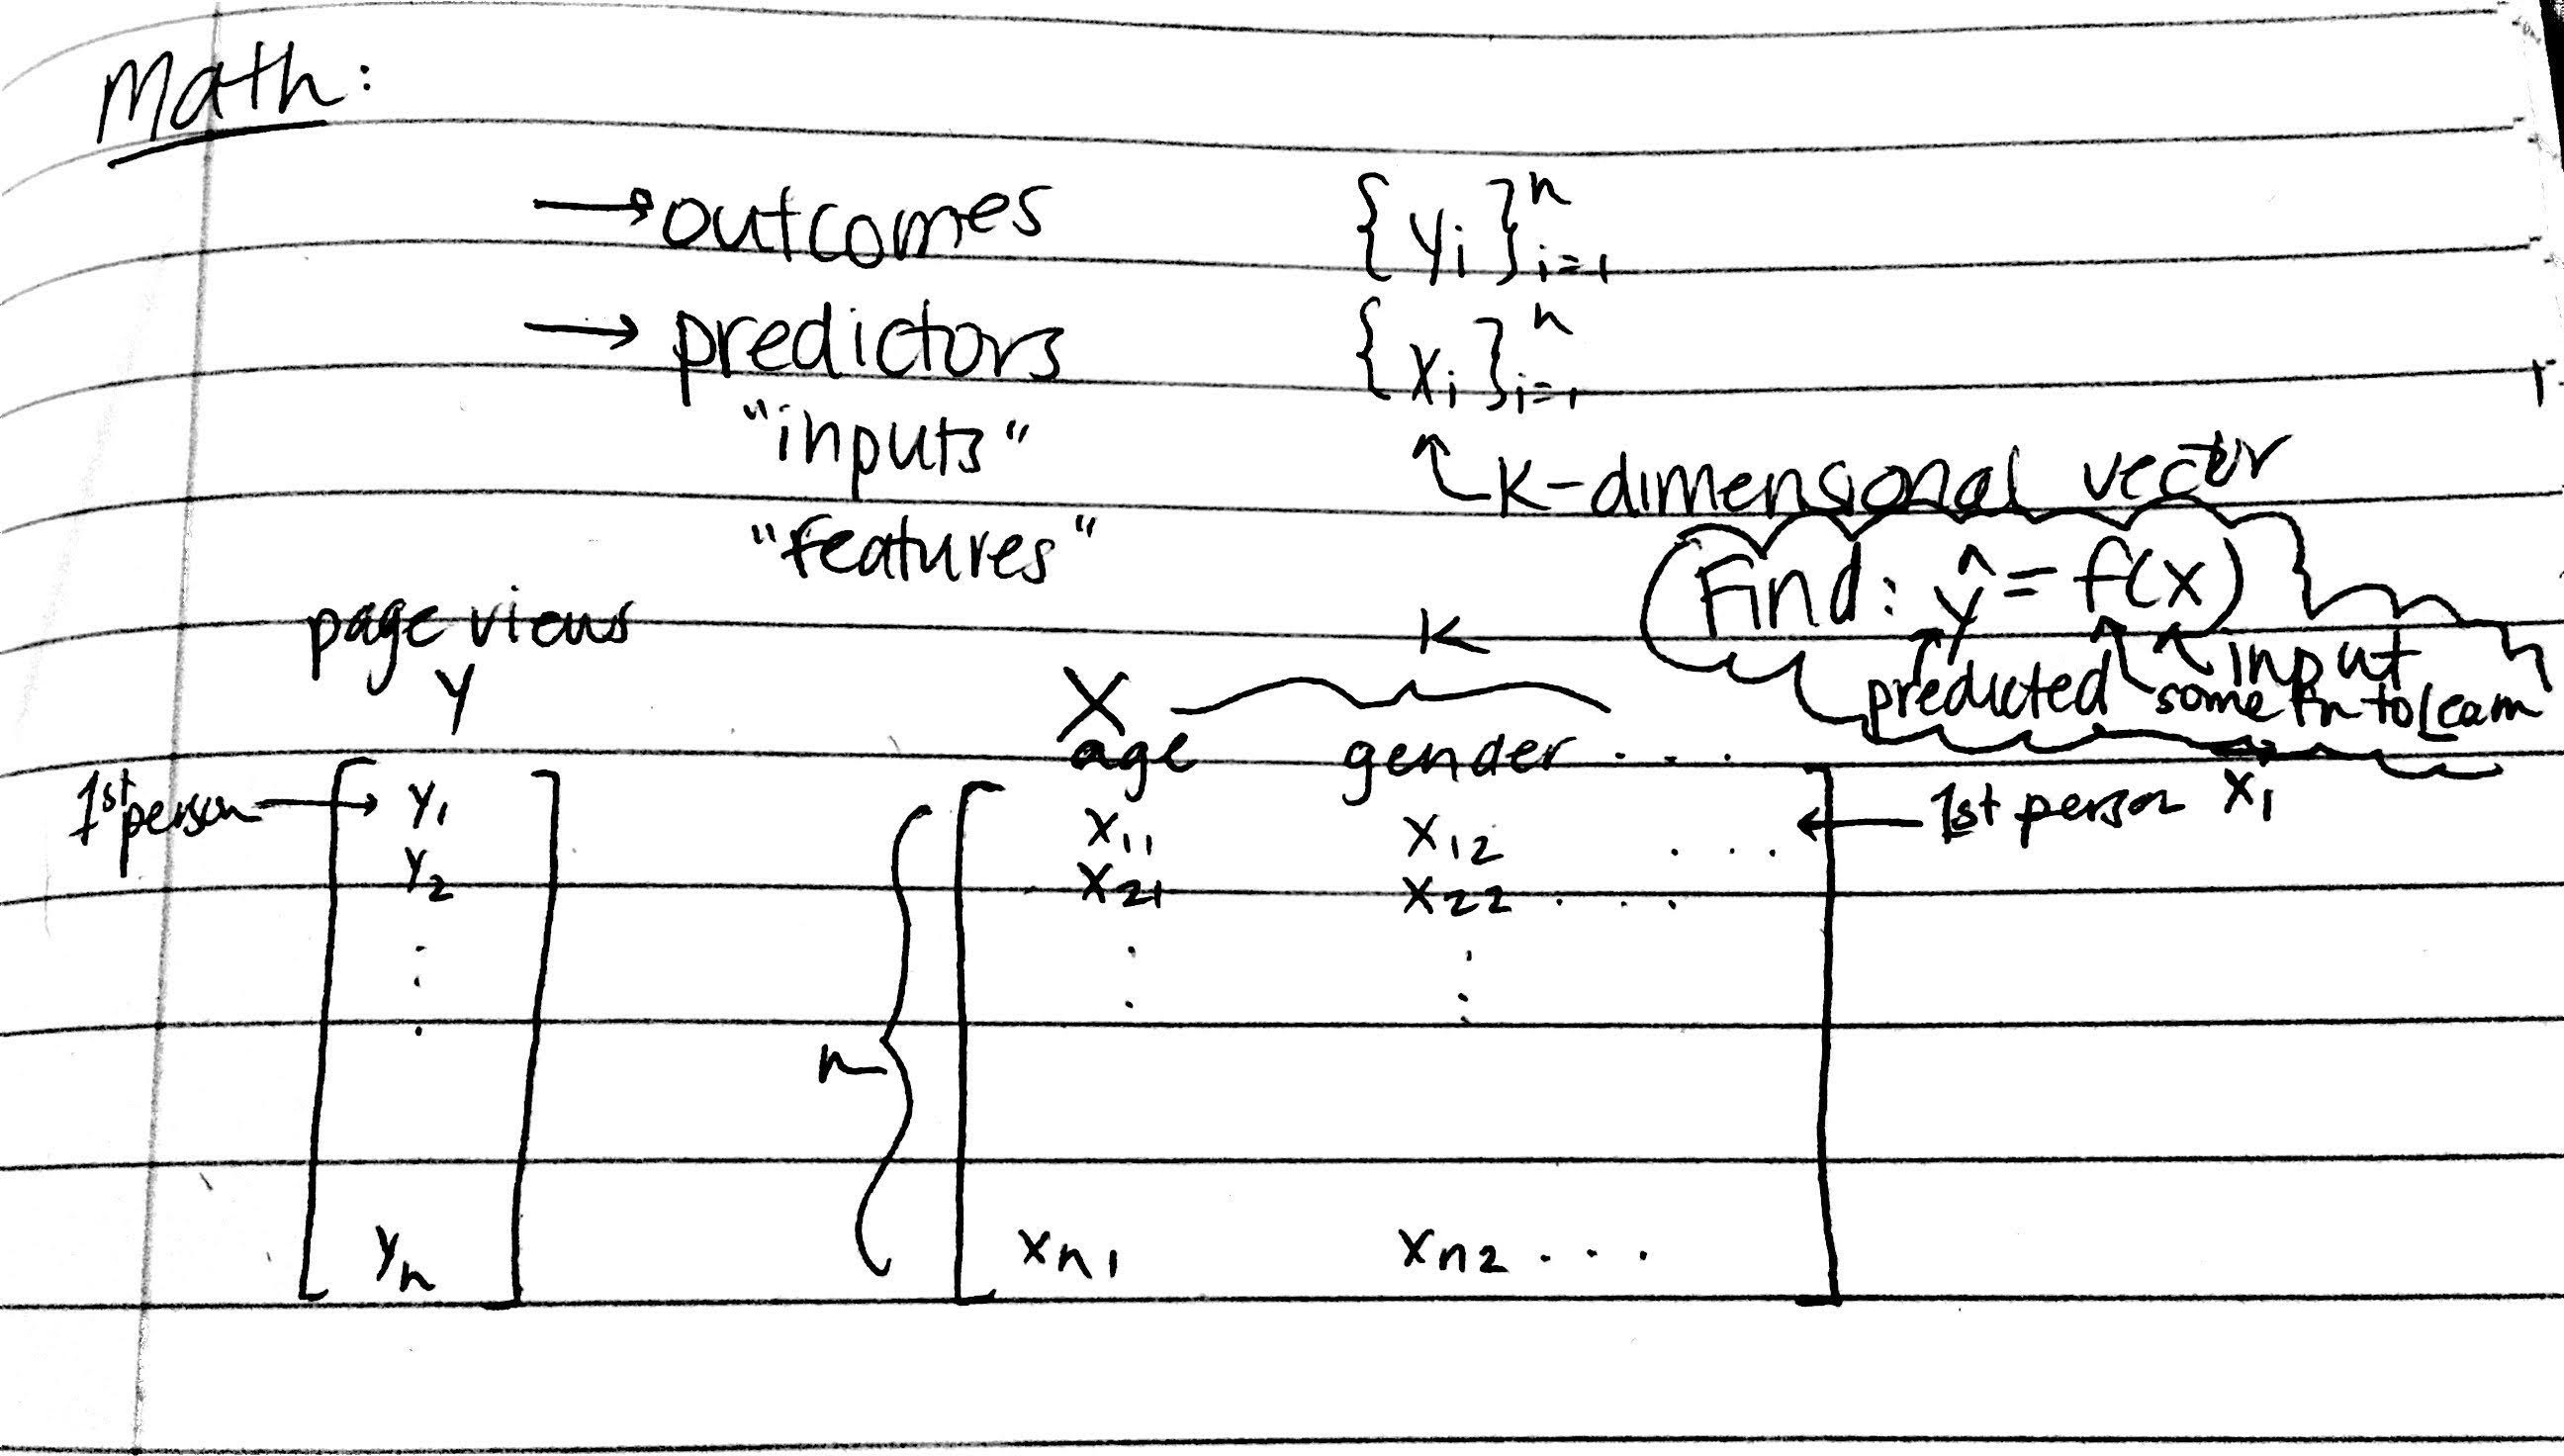
\includegraphics[width=\textwidth]{figures/fig1.jpg}
    \caption{ Representing the data for Section Math}
   \end{center}
\end{figure}

\subsection{Maximum Likelihood}:

Assume some family of probabilistic model generated the data. Find the model under which the observed data are most likely.\\

f*  = argmax\textsubscript{f} P($D|f$) \\

Common assumption : y =f(x\textsubscript{i}) + E\textsubscript{i} \\

P($E\textsubscript{i} | f$) = P($y\textsubscript{i} -f(x\textsubscript{i}) | f $)\\

 =  (1 / $\sqrt{\mathstrut}$ $2\pi\sigma^2$ ) * exp\textsuperscript{(-1/$2\sigma^2$)*(y\textsubscript{i} -f(x\textsubscript{i}))\textsuperscript{2} }\\
 \begin{equation}
	P(D|f)=   \prod\limits_{i=1}^n P(D\textsubscript{i}|f)
\end{equation}
\begin{equation}
	P(D|f)=   \prod\limits_{i=1}^n (1 / \sqrt{\mathstrut} 2\pi\sigma^2 ) * exp\textsuperscript{(-1/2$\sigma^2$)*(y\textsubscript{i} -f(x\textsubscript{i}))\textsuperscript{2} }\end{equation}
	
Simplifying Likelihood Fn.

\begin{equation}
	P(D|f)=    (2\pi\sigma^2)\textsuperscript{-n/2}  * exp( -1/2 \sigma^2 *\sum\limits_{i=1}^n (y\textsubscript{i} -f(x\textsubscript{i}))\textsuperscript{2})
	 \end{equation}
	 
\begin{equation}
Log P(D|f)=   -n/2 * (2\pi\sigma^2)   - 1/2 \sigma^2 *\sum\limits_{i=1}^n (y\textsubscript{i} -f(x\textsubscript{i}))\textsuperscript{2}
	\end{equation}

Maximizing squared loss = maximising (log) likelihood, assuming additive gaussian noise. (errors are normally distributed) \\

Choice for f: \^{y} = f(x) = w.X = w\textsubscript{1}x\textsubscript{1} + w\textsubscript{2}x\textsubscript{2} +... + w\textsubscript{n}x\textsubscript{n}

 \begin{equation}
	w\textsuperscript{*} = argmin\textsubscript{w}   \sum\limits_{i=1}^n (y\textsubscript{i} - w.x\textsubscript{i})
\end{equation}

\begin{figure}[ht]
  \begin{center}
    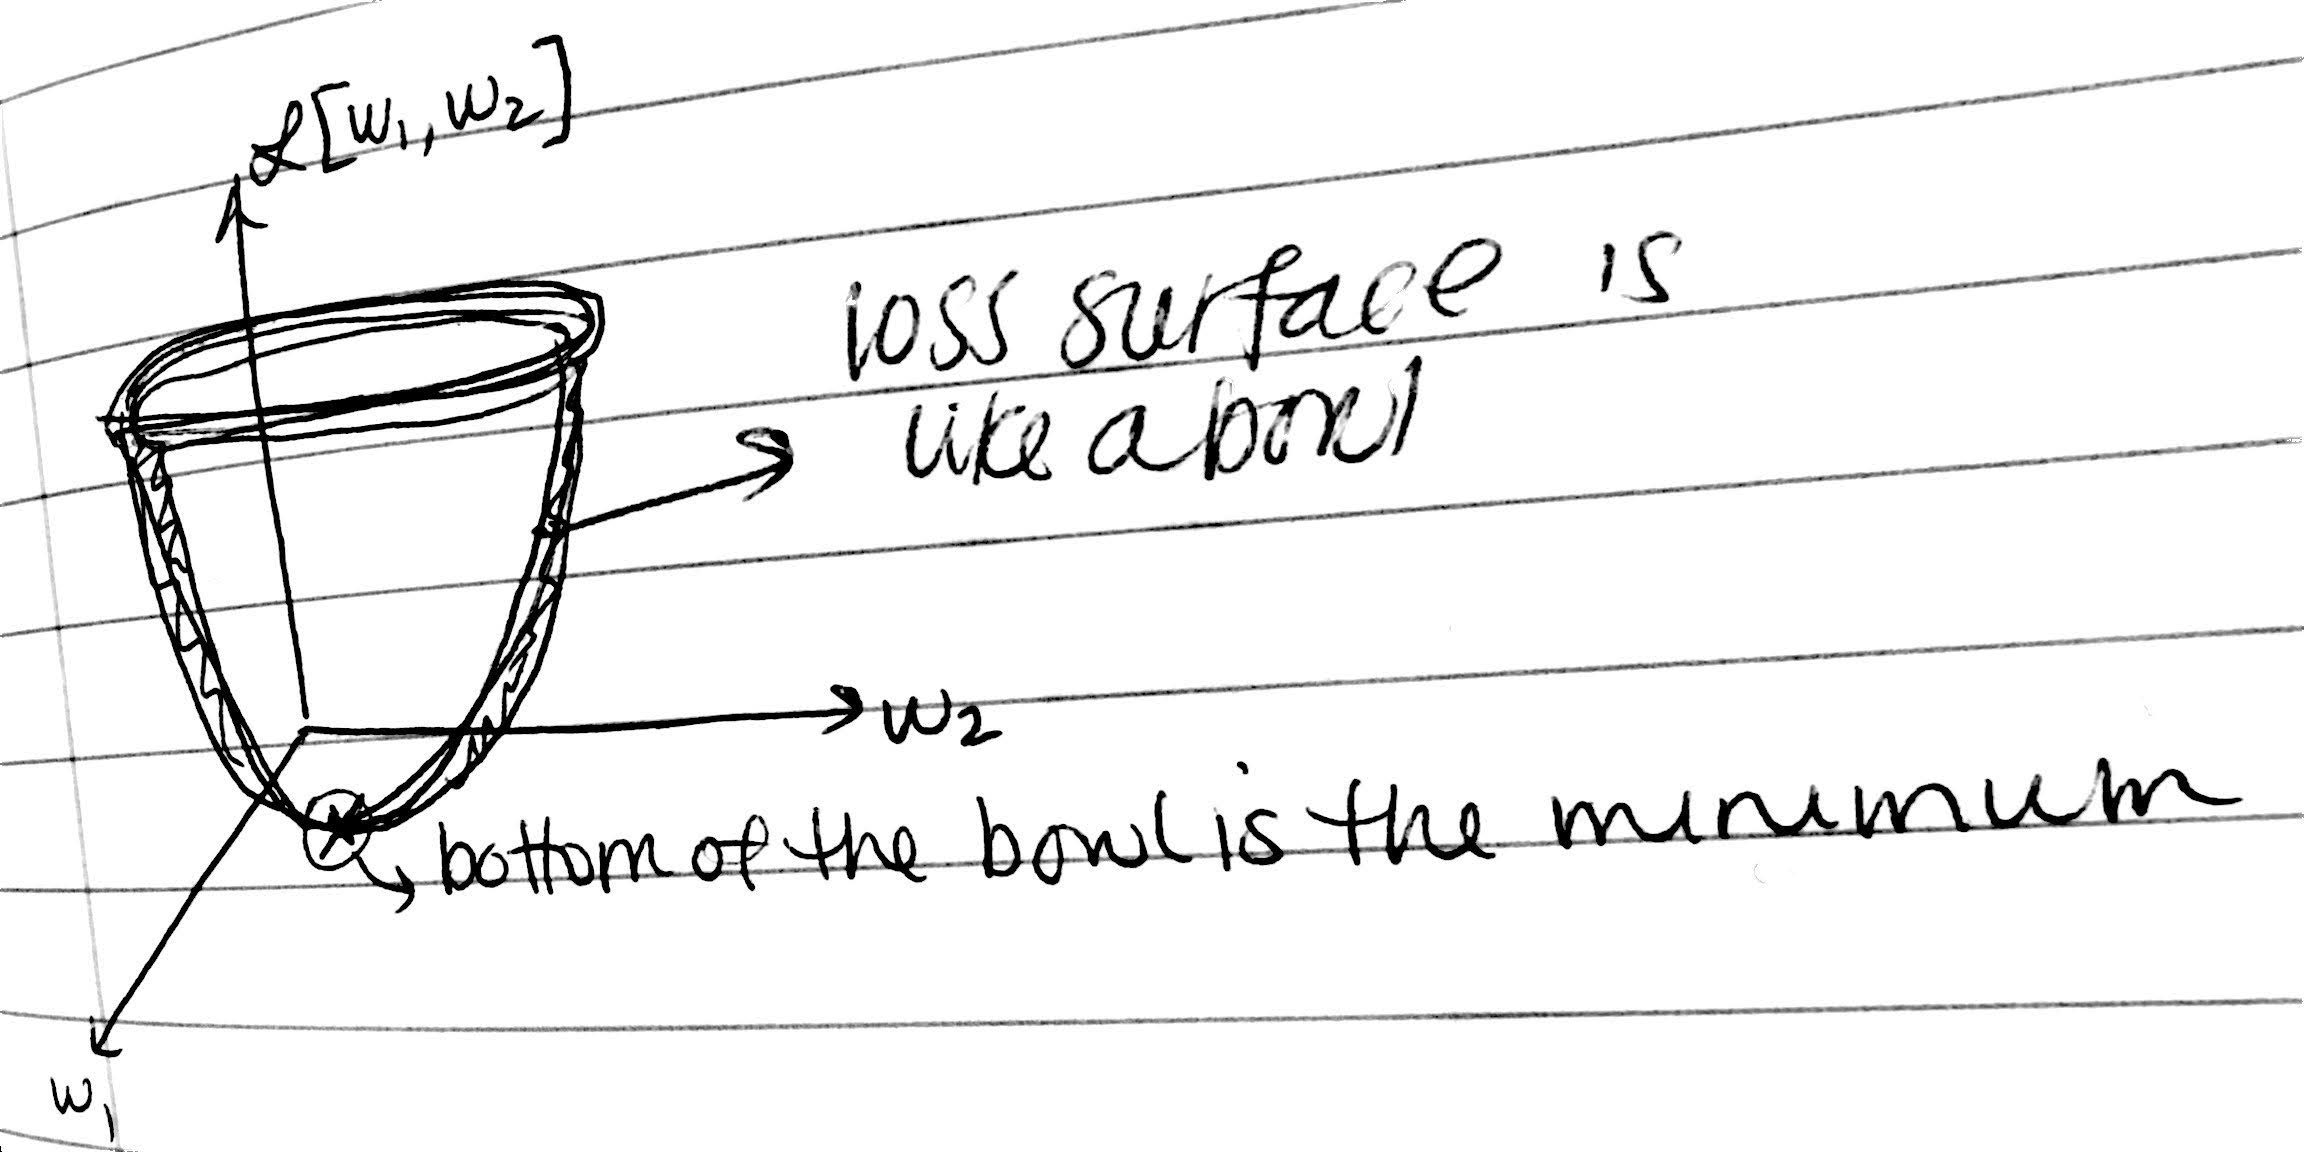
\includegraphics[width=\textwidth]{figures/fig2.jpg}
    \caption{ Loss Surface}
   \end{center}
\end{figure}

Loss Surface is easy to visualise in 2D, difficult with high dimensions. One shouldnt do a manual search for the bottom of the loss surface

\begin{equation}
	L[f] = 1/ N *  \sum\limits_{i=1}^n (y\textsubscript{i} - w.x\textsubscript{i})^2
\end{equation}

Differentiating -(8) wrt w and equating with 0.

\begin{equation}
	0 = -2/ N *  \sum\limits_{i=1}^n (y\textsubscript{i} - w.x\textsubscript{i})x\textsubscript{i}
\end{equation}

Equation -(9) can be written in vectorized notation as :

\begin{equation}
	0 =  X\textsuperscript{T} * (y - Xw)
\end{equation}

Simplifying:\\

\^{w} =  (X\textsuperscript{T}X)\textsuperscript{-1}X\textsuperscript{T}y \\

\^{w} is the best estimate of w. Time complexity to find \^{w} is O(NK\textsuperscript{2} + K\textsuperscript{3}) \\

If the data is very wide, this would be very time consuming. 

\subsection{Gradient Descent}
WRT to Loss Surface
\begin{enumerate}
  \item Start somewhere random
  \item Follow the negative gradient to the bottom of the surface.
\end{enumerate}


w = w - eta * (gradient)

gradient is same as equation - (9)\\

eta is the step size: large = big steps, small = slow progression \\
Computational Costs:\\
Xw = O(KN)\\
Y-Xw=O(N)\\
X\textsuperscript{T}(Y-Xw) =O(KN)\\
Time Complexity is O(KN + N + KN) = O(KN)\\

Gradient Descent would be better for higher dimension.

\subsection{Stochastic Gradient Descent}

Same intuition ( follow the gradient) but follow the approximate gradient.

\begin{equation}
	gradient of Loss function (dL/dw)= -2/ N *  \sum\limits_{i=1}^n (y\textsubscript{i} - w.x\textsubscript{i})x\textsubscript{i}
\end{equation}

Take a random sample n very very small as compared to N examples to estimate the gradient.

\begin{equation}
	gradient of Loss function (dL/dw)= -2/ n *  \sum\limits_{i=1}^n (y\textsubscript{i} - w.x\textsubscript{i})x\textsubscript{i}
\end{equation}

Time Complexity is O(KN + N + KN) = O(KN) \\

On avg you are correct + close to the bottom. Choosing eta becomes tricky, make it smaller as you go closer to convergence

\subsection{2nd order derivative}

In methods like newton method,  second order derivative of loss function is calculated to determine the curvature of the surface. More computation to take 2nd order derivative but saves time to reach to minimum. Faster steps on flatter surface and smaller steps on steep surface.

\subsection{Some Additional Points}

\begin{enumerate}
  \item In highly skewed data, used median over mean.
  \item Median and Geometric Mean in log scale are pretty close.
  \item Log scale is preferred while working with heavy tail distribution.
\end{enumerate}


















